There are multiple ways a computer can communicate with its peripheral devices.
The most used techniques are Memory-Mapped I/O (MMIO) and Port-Mapped I/O
(PMIO). Port-Mapped I/O s an older method of accessing peripherals, and is much
more common in consumer computers with Intel or AMD CPUs\cite{intelmanual}.\\
PMIO requires the processor to have additional pins and special instructions,
just for communication with I/O devices. I/O devices have a specified port
number, which the processor uses to identify and communicate with the device.
For example, Intel x86 processors might communicate with a keyboard, using the
special \texttt{in} instruction, specifying keyboard ID
\texttt{0x60}\cite{intel:pch}\cite{osdev:io_ports}:
\begin{lstlisting}[language={[x86masm]Assembler}]
_wait:
  in  al, 64H   ; Read status of device 0x64
  and al, 1     ;
  jz  _wait	; Check if ready to read
  in  al, 60H   ; Read data
\end{lstlisting}
Besides the added circuitry in the processor, port-mapped I/O are fairly
simple to implement and easy to use. They have their own special instructions,
and they do not share memory space, which prevents confusion about
memory segmenting.
However, PMIO approach is very limited to only \texttt{in} and \texttt{out}
instructions, as well as very limited "ID" space for the devices.\\

Memory-Mapped I/O is commonly used by RISC architectures. In MMIO,
communication with the peripherals happens over the same address bus as the
memory, so that memory and I/O communication share address space.
\\
TO BE FINISHED
\\


MIPS sees Input/Output (IO) devices as a set of special-purpose registers. These
special registers are the processors only way of communicating with a given
device.\\
For every device, there 3 types of registers\cite{cs_uwm:memory_mapped_io}:
\begin{itemize}
	\item \texttt{Status registers}\\
	Provide information about the underlying device. These registers are
	read-only for the CPU.

	\item \texttt{Control registers}\\
	Used to communicate and control the device. These registers are
	writeable for the CPU, but may not always be readable.

	\item \texttt{Data registers}\\
	Used for the actual data-transport. For example, the latest key pressed
	on the keyboard might be stored in this register.
\end{itemize}

In memory, these registers have allocated 4 bytes each, and are always located
sequentially in the memory. Figure \ref{fig:io_registers} shows the actual bit-allocation in the register.
\begin{figure}[H]
	\centering
	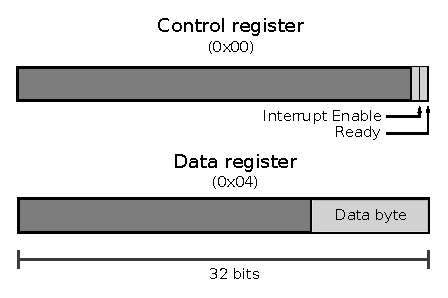
\includegraphics[scale=1]{io/io_registers.eps}
	\caption{Set of memory mapped I/O registers}
	\label{fig:io_registers}
\end{figure}

When a device is detected, both the CPU and the device will retrieve a set of
these paired registers. From now on, it is up to the driver to interface with
the devices.\\
Depending on the type of the IO device, the device can be represented from a
few registers to dozens. For example, a mouse or a keyboard only transmits few
bytes of information at a time, needing only a few registers, while graphic
adaptors or disk drives might need more\cite{cs_uwm:memory_mapped_io}.\\
These special-purpose registers are located in the RAM, mapped to a certain
segment. A device controller maintains a list of these registers, and maps new
devices to the memory.\cite{britton:mips}\\
On MIPS32, the highest 64 kilobytes (\texttt{0xffff0000 - 0xffffffff}) in the
available memory are used for mapping these special registers\cite{cs_uwm:memory_mapped_io}.
The memory mapping the IO area must not be cached, as it can cause major problems
for the caches, and heavy delays due to many cache-misses\cite{see_mips_run}.



\subsection{Implementation}
Implementation of external devices requires a lot of new modules and features
in the simulator. The main issue is that we require to communicate with
events, not handled by the simulator. To achieve this, we will use first-in
first-out special files (FIFO), more commonly known as named pipes. This pipes
will serve as a communication channels to external devices (or rather, external
programs).

\subsection{Named pipes}
For every unique device available, the simulator will create a named pipe,
using which these two will communicate.

\begin{lstlisting}[language=c]
/* Simulator pipe structure */
typedef struct pipe_io {
	bool ready;
	bool interrupt_enable;
	uint8_t byte;
} pipe_io_t;

\end{lstlisting}
